\chapter{Implementação e Testes}
\label{chap:imp-test}

\section{Introdução}
\label{chap4:sec:intro}
Após a fundamentação teórica, este capítulo descreve a materialização prática do sistema de deteção de anomalias para redes \ac{IoT}. O foco incide sobre a criação de um \textit{dataset} equilibrado, o tratamento de discrepâncias estatísticas e a avaliação de quatro modelos de Inteligência Artificial: \ac{XGBoost}, \ac{LightGBM}, Random Forest e \ac{MLP}. O capítulo encontra-se organizado da seguinte forma: a Secção \ref{chap4:sec:preproc} detalha o pré-processamento de dados; a Secção \ref{chap4:sec:treino} descreve a metodologia de treino e persistência; a Secção \ref{chap4:sec:filtragem} apresenta o mecanismo de filtragem ativa e mitigação automática de ameaças; a Secção \ref{chap4:sec:simulacao} expõe o ambiente de simulação em tempo real; a Secção \ref{chap4:sec:resultados} elabora a análise rigorosa das métricas em ambiente \textit{Zero-Day}; e, por fim, a Secção \ref{chap4:sec:concs} apresenta a decisão final.

\section{Pré-processamento e Engenharia de Dados}
\label{chap4:sec:preproc}
A eficácia da deteção depende da qualidade dos dados. Utilizou-se o dataset CICIoT2023, consolidando os volumes Merged01 a Merged05 para garantir uma base de amostragem rica para treino dos modelos e Merged06 a Merged10 para validação dos modelos treinados.

Numa primeira tentativa, verificou-se que treinar a Inteligência Artificial exclusivamente com assinaturas de anomalias induzia um viés (bias) extremo no modelo, resultando num fenómeno de over-triggering (taxa de Falsos Positivos próxima de 100\% face a utilizadores legítimos). Para mitigar este problema, procedeu-se à extração de um dataset de treino equilibrado com mais de 80.000 amostras, garantindo a integração de 10.000 instâncias de tráfego benigno (Normal).

\subsection{Categorização de Anomalias e Rotulagem}

Para que o sistema de monitorização seja capaz de atuar de forma precisa,
a Inteligência Artificial foi treinada para identificar nove categorias
distintas de anomalias :

\begin{itemize}
    \item \textbf{Ataques Volumétricos TCP} (\textit{DDoS-TCP} e
    \textit{DoS-TCP}): inundação maliciosa de pedidos de sincronização
    TCP, mitigada através da injeção de regras \texttt{iptables} com
    ação \texttt{DROP} sobre o protocolo TCP do IP atacante;

    \item \textbf{Ataques Volumétricos UDP/ICMP} (\textit{DDoS-UDP/ICMP}
    e \textit{DoS-UDP/ICMP}): estrangulamento de largura de banda por
    inundação de datagramas e pacotes de controlo, mitigado com bloqueio
    simultâneo de tráfego UDP e ICMP ;

    \item \textbf{Ameaças de IoT Múltiplo} (\textit{Mirai Botnet}):
    comprometimento total do dispositivo de origem por malware de botnet,
    mitigado com isolamento completo do IP atacante sem filtragem de
    protocolo (\texttt{DROP} absoluto);

    \item \textbf{Quebra de Senha} (\textit{BruteForce}): tentativas
    automatizadas de acesso por força bruta, tipicamente dirigidas à
    porta 22 (SSH), mitigadas com \texttt{REJECT} focado no protocolo
    TCP e nessa porta específica;

    \item \textbf{Reconhecimento} (\textit{Recon}): varrimento furtivo
    da rede para mapeamento de dispositivos e serviços ativos, detetado
    através de padrões estatísticos de fluxo;

    \item \textbf{Falsificação} (\textit{Spoofing}): falsificação de
    endereços IP ou MAC para obtenção de acesso não autorizado, mitigada
    com isolamento completo do IP de origem (\texttt{DROP} absoluto).
\end{itemize}

A ação de mitigação específica aplicada a cada classe é executada
autonomamente pelo módulo de filtragem ativa, detalhado na
Secção~\ref{chap4:sec:filtragem}.

\subsection{O Papel dos Label Encoders}
Os algoritmos de \textit{Machine Learning} são baseados em equações matemáticas que operam exclusivamente com números. Por este motivo, é impossível entregar ao modelo categorias em formato de texto como "\ac{DDoS}-\ac{TCP}". O \texttt{LabelEncoder} atua como um dicionário de tradução bidirecional, mapeando cada ataque único para um índice numérico (ex: 'DDoS-TCP' $\rightarrow$ 2). Este tradutor é guardado num ficheiro \textit{.pkl} para que, em ambiente de produção, o Router possa converter o número previsto pela IA de volta para um nome legível por humanos e sistemas de segurança.

\subsection{Filtro de Pureza e Normalização}
Identificou-se a presença de valores infinitos (\texttt{np.inf}) em métricas de volumetria, resultantes de anomalias na captura. Implementou-se um filtro que substituiu estes valores por zero, garantindo que algoritmos como o Random Forest não falhassem na compilação geométrica das matrizes. Para o \ac{MLP}, aplicou-se o \texttt{StandardScaler} para normalizar a escala dos dados, evitando que variáveis com grandes magnitudes dominassem injustamente o treino.


\section{Metodologia de Treino e Persistência}
\label{chap4:sec:treino}
Os modelos foram treinados utilizando o "Dataset de Treino" equilibrado. O Excerto de Código \ref{lst:treino_ciber} ilustra a rotina de treino e exportação do modelo \ac{LightGBM}.

\begin{lstlisting}[language=Python, caption={Rotina de treino e persistência do modelo LightGBM.}, label={lst:treino_ciber}]
import pandas as pd
import lightgbm as lgb
import joblib

# 1. Carregar Dataset equilibrado
df = pd.read_csv('dataset_treino.csv')

# 2. Preparar X e y
y = df['label_encoded']
X = df.drop(['Label', 'label_encoded', 'categoria'], axis=1)

# 3. Treino do modelo focado em Edge
modelo = lgb.LGBMClassifier(n_estimators=100, random_state=42)
modelo.fit(X, y)

# 4. Guardar cerebro para o Router
joblib.dump(modelo, 'modelo_ciberseguranca_lgbm.pkl')
\end{lstlisting}


\section{Mecanismo de Filtragem}
\label{chap4:sec:filtragem}

A deteção atempada de uma anomalia através de algoritmos de \textit{Machine Learning} constitui apenas a primeira fase de Sistema de Prevenção de Intrusões (IPS). Para que a infraestrutura de \textit{Edge Computing} garanta a resiliência da \textit{Smart City}, é imperativo que a inferência preditiva seja traduzida, em milissegundos, numa ação de bloqueio ao nível da rede. Este capítulo detalha a arquitetura de mitigação ativa desenvolvida, assente na manipulação dinâmica das tabelas de encaminhamento do \textit{kernel} do sistema operativo através da ferramenta \texttt{iptables}.

Em vez de depender de soluções de \textit{Firewall} externas de elevado custo, o nó \textit{Edge} foi programado para atuar autonomamente, convertendo a saída do modelo numa regra de bloqueio estrita. A função de mitigação foi estruturada para ser granular, aplicando o princípio do menor privilégio: a penalização aplicada ao endereço de \ac{IP} atacante é talhada à medida da classe de anomalia detetada, garantindo máxima eficácia com o mínimo impacto colateral.

A lógica de atuação do sistema obedece às seguintes regras de contenção:

\begin{itemize}
    \item \textbf{Ataques Volumétricos TCP (\ac{DDoS}-\ac{TCP} e \ac{DoS}-\ac{TCP}):}
    Quando a rede é inundada por pedidos de sincronização maliciosos, o sistema invoca uma regra \texttt{iptables} que descarta silenciosamente (\texttt{DROP}) pacotes cujo protocolo seja estritamente \ac{TCP} provenientes daquele \ac{IP}. O uso da ação \texttt{DROP} (em vez de \texttt{REJECT}) é vital em cenários volumétricos, pois evita que o \textit{router} desperdice poder computacional a enviar mensagens de "conexão recusada" de volta ao atacante.

    \item \textbf{Ataques Volumétricos UDP/ICMP (\ac{DDoS}-\ac{UDP}/\ac{ICMP} e \ac{DoS}-\ac{UDP}/\ac{ICMP}):}
    De forma análoga aos ataques \ac{TCP}, a identificação destas classes gera duas regras em simultâneo: o bloqueio transversal de tráfego de datagramas (\ac{UDP}) e o bloqueio de tráfego de controlo e testes de eco (\ac{ICMP}), anulando táticas comuns de estrangulamento de largura de banda, como os \textit{Ping Floods}.

    \item \textbf{Ameaças de IoT Múltiplo e Falsificação (\textit{Mirai} e \textit{Spoofing}):}
    Ataques orquestrados por \textit{Botnets} como o \textit{Mirai} representam um comprometimento total do dispositivo de origem. Como tal, o sistema aplica uma regra absolutista (\texttt{DROP} sem filtragem de protocolo), isolando por completo o \ac{IP} atacante da rede, impedindo que este comunique com o exterior ou tente propagar o \textit{malware} internamente na \textit{Smart City}.

    \item \textbf{Quebra de Senha (\textit{BruteForce}):}
    Ao detetar uma tentativa de força bruta (normalmente direcionada a serviços de administração remota), o sistema foca o bloqueio especificamente no protocolo \ac{TCP} e na porta \texttt{22} (serviço SSH). Adicionalmente, utiliza-se a ação \texttt{REJECT}. Esta resposta envia ativamente um pacote de recusa ao atacante, quebrando imediatamente a ferramenta automatizada de tentativa de \textit{passwords}, fechando a porta sem interromper outro possível tráfego legítimo.
\end{itemize}

\subsection{Implementação Algorítmica}
\label{chap4:sec:implementacao}
O Excerto de Código \ref{lst:mitigacao} ilustra o \textit{script} Python encarregue de orquestrar a \textit{Blacklist} dinâmica. A função \texttt{aplicar\_mitigacao} atua como uma ponte entre a camada lógica (Inteligência Artificial) e a camada física (Camada de Rede).

\begin{lstlisting}[language=Python, caption={Lógica de Mitigação Ativa baseada em \texttt{iptables}.}, label={lst:mitigacao}]
def aplicar_mitigacao(classe, ip_atacante, tempo_ms):
    if classe in ['DDoS-TCP', 'DoS-TCP']:
        executar_comando(f"iptables -A INPUT -p tcp -s {ip_atacante} -j DROP")

    elif classe in ['DDoS-UDP/ICMP', 'DoS-UDP/ICMP']:
        executar_comando(f"iptables -A INPUT -p udp -s {ip_atacante} -j DROP")
        executar_comando(f"iptables -A INPUT -p icmp -s {ip_atacante} -j DROP")

    elif classe == 'Mirai-Botnet' or classe == 'Spoofing':
        executar_comando(f"iptables -A INPUT -s {ip_atacante} -j DROP")

    elif classe == 'BruteForce':
        executar_comando(f"iptables -A INPUT -p tcp --dport 22 -s {ip_atacante} -j REJECT")

    # Auditoria e Registo de Desempenho
    print(f"-->Mitigacao aplicada para: {classe} (IP: {ip_atacante}) - Tempo de IA: {tempo_ms:.2f} ms")
\end{lstlisting}

Por fim, cada intervenção do \textit{Edge Router} gera um evento de auditoria no \textit{log} do sistema (incluindo o \ac{IP} isolado, o tipo de ameaça e o custo de inferência algorítmica). Estes registos comprovam que o ciclo completo de defesa --- desde a leitura do pacote, inferência pela rede neuronal e injeção da regra de bloqueio --- decorre nos exigentes limites impostos pelo paradigma de operações em tempo real.


\section{Ambiente de Simulação em Tempo Real}
\label{chap4:sec:simulacao}

Para validar a viabilidade dos modelos de \textit{Machine Learning} num cenário realista de \textit{Edge Computing}, construiu-se uma topologia de rede virtualizada com recurso à ferramenta Mininet. De forma a refletir a complexidade de uma infraestrutura autêntica, a arquitetura foi composta por três elementos fundamentais: um nó atacante (h1), responsável pela injeção em massa dos pacotes provenientes do \textit{dataset} de validação (via protocolo UDP); um router central; e um servidor dedicado de análise (h2), atuando como nó \textit{Edge} de Inteligência Artificial.

Nesta topologia, o tráfego injetado por h1 atravessa o router central, que está configurado para redirecionar o fluxo de rede para o servidor h2. É neste nó \textit{Edge} que ocorre a interceção dos pacotes, a extração de \textit{features} em tempo real e a submissão do tráfego à inferência do modelo treinado. Ao separar o encaminhamento básico (router) do processamento analítico (h2), este ambiente de \textit{stress-test} permitiu simular não apenas a eficácia da classificação lógica do modelo, mas sobretudo as restrições físicas inerentes a uma rede em produção, tais como a latência imposta pelo redirecionamento, engarrafamentos de \textit{buffer} e as inevitáveis perdas de pacotes.

Na Figura \ref{fig:representacaomininet}, é possível observar a arquitetura montada no Mininet.

\begin{figure}[H]
    \centering
    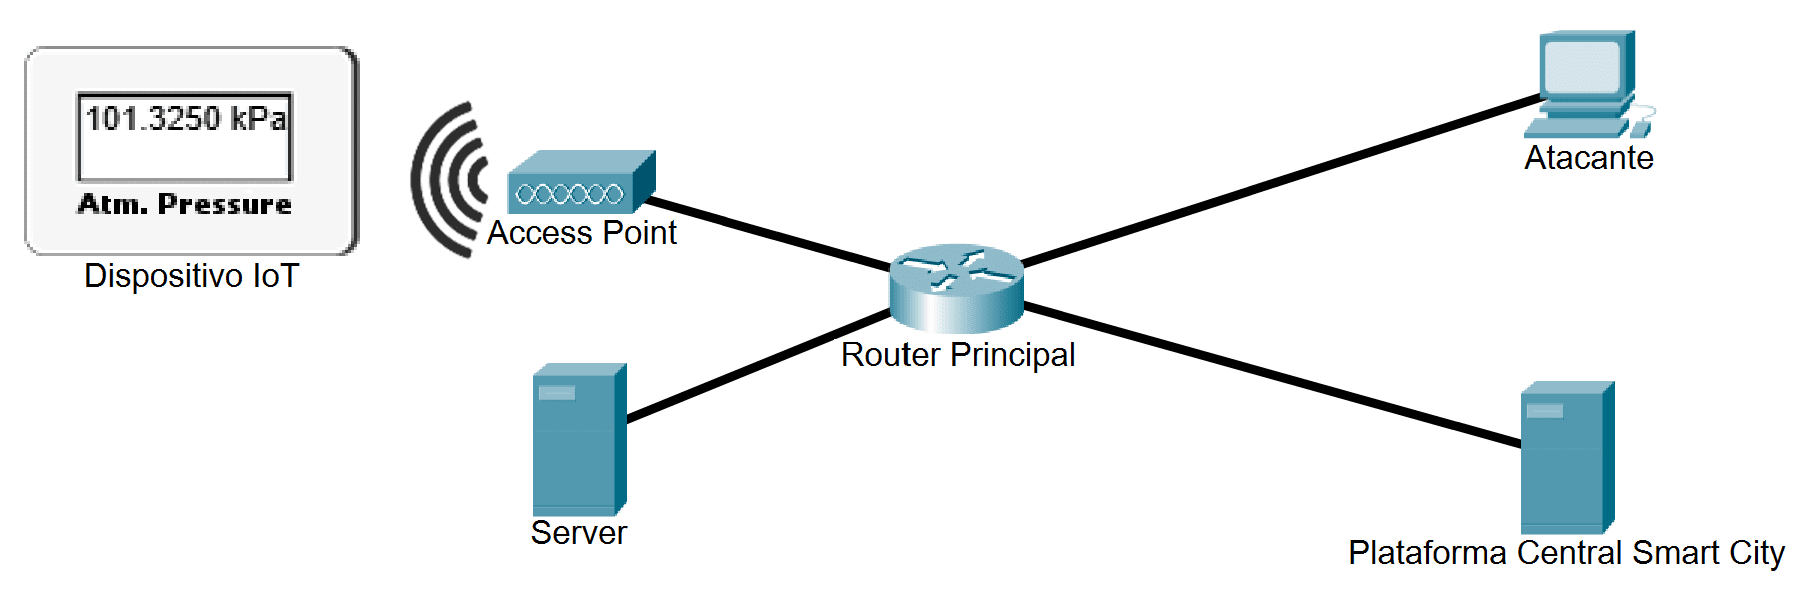
\includegraphics[width=0.9\textwidth]{imagens/IoT Device.png}
    \caption{Arquitetura montada no Mininet.}
    \label{fig:representacaomininet}
\end{figure}

\section{Resultados e Otimização da Mitigação}
\label{chap4:sec:resultados}

\subsection{Mecanismo de Filtragem Rápida via Blacklist Dinâmica}
\label{chap4:sec:blacklist}
Apesar do baixo tempo de inferência alcançado pelo modelo MLP ($\sim$1 ms), submeter a totalidade do tráfego volumétrico de um ataque DDoS (milhões de pacotes) à análise da Inteligência Artificial resultaria no esgotamento prematuro do processador do \textit{Edge Router}. Para contornar esta limitação arquitetural, foi implementado um sistema de mitigação híbrido com recurso a uma \textit{Blacklist} Dinâmica.

O fluxo de funcionamento dita que apenas os pacotes iniciais de uma origem desconhecida são sujeitos à carga computacional da inferência por \textit{Machine Learning}. No momento em que a rede neuronal sinaliza um IP de origem como malicioso, esse endereço é imediatamente adicionado a uma tabela de bloqueio (em memória \textit{cache}). Consequentemente, os milhares de pacotes subsequentes desse atacante são descartados de forma instintiva (\textit{drop}) nas camadas primárias da infraestrutura de rede lidas em tempo real, contornando o \textit{pipeline} da IA. Esta simbiose entre inteligência preditiva e filtragem tradicional baseada em regras conferiu ao sistema uma escalabilidade formidável face a injeções de tráfego de alta densidade.

\subsection{Métricas de Avaliação}
Para quantificar o sucesso preditivo e a viabilidade operacional dos modelos em ambiente de \textit{Edge Computing}, utilizou-se um conjunto de quatro métricas fundamentais:
\begin{itemize}
    \item \textbf{Accuracy Global:} Representa a percentagem total de pacotes corretamente classificados pelo modelo. Embora intuitiva, pode ser enganosa em dados desbalanceados.
    \item \textbf{F1-Score Ponderado:} É a média harmónica entre a Precisão (falsos alarmes) e o \textit{Recall} (capacidade de apanhar o \textit{hacker}). Esta métrica é o indicador real de robustez, pois penaliza modelos que ignoram ataques raros.
    \item \textbf{Tempo Médio de Inferência (Latência):} Avalia o tempo, em milissegundos (ms), que o modelo demora a processar os dados de um pacote e a emitir uma decisão de bloqueio ou permissão. Numa arquitetura IoT, uma latência de processamento o mais próxima possível de 1 milissegundo é crítica para evitar o esgotamento do \textit{buffer} do \textit{router} e garantir a fluidez da rede.
    \item \textbf{Estabilidade da Latência (Variância / Jitter):} Analisada através de diagramas de dispersão estatística (\textit{Boxplot}), avalia a consistência do tempo de resposta ao longo do teste. Modelos com alta variabilidade apresentam picos de latência imprevisíveis que, durante ataques volumétricos, resultariam no colapso do tráfego legítimo por incapacidade momentânea de processamento.
\end{itemize}

\subsection{Análise do Desempenho Global}
\label{chap4:sec:desempenho_global}

A Figura \ref{fig:teste_cego_global} apresenta a comparação das métricas globais entre os modelos avaliados.

\begin{figure}[H]
    \centering
    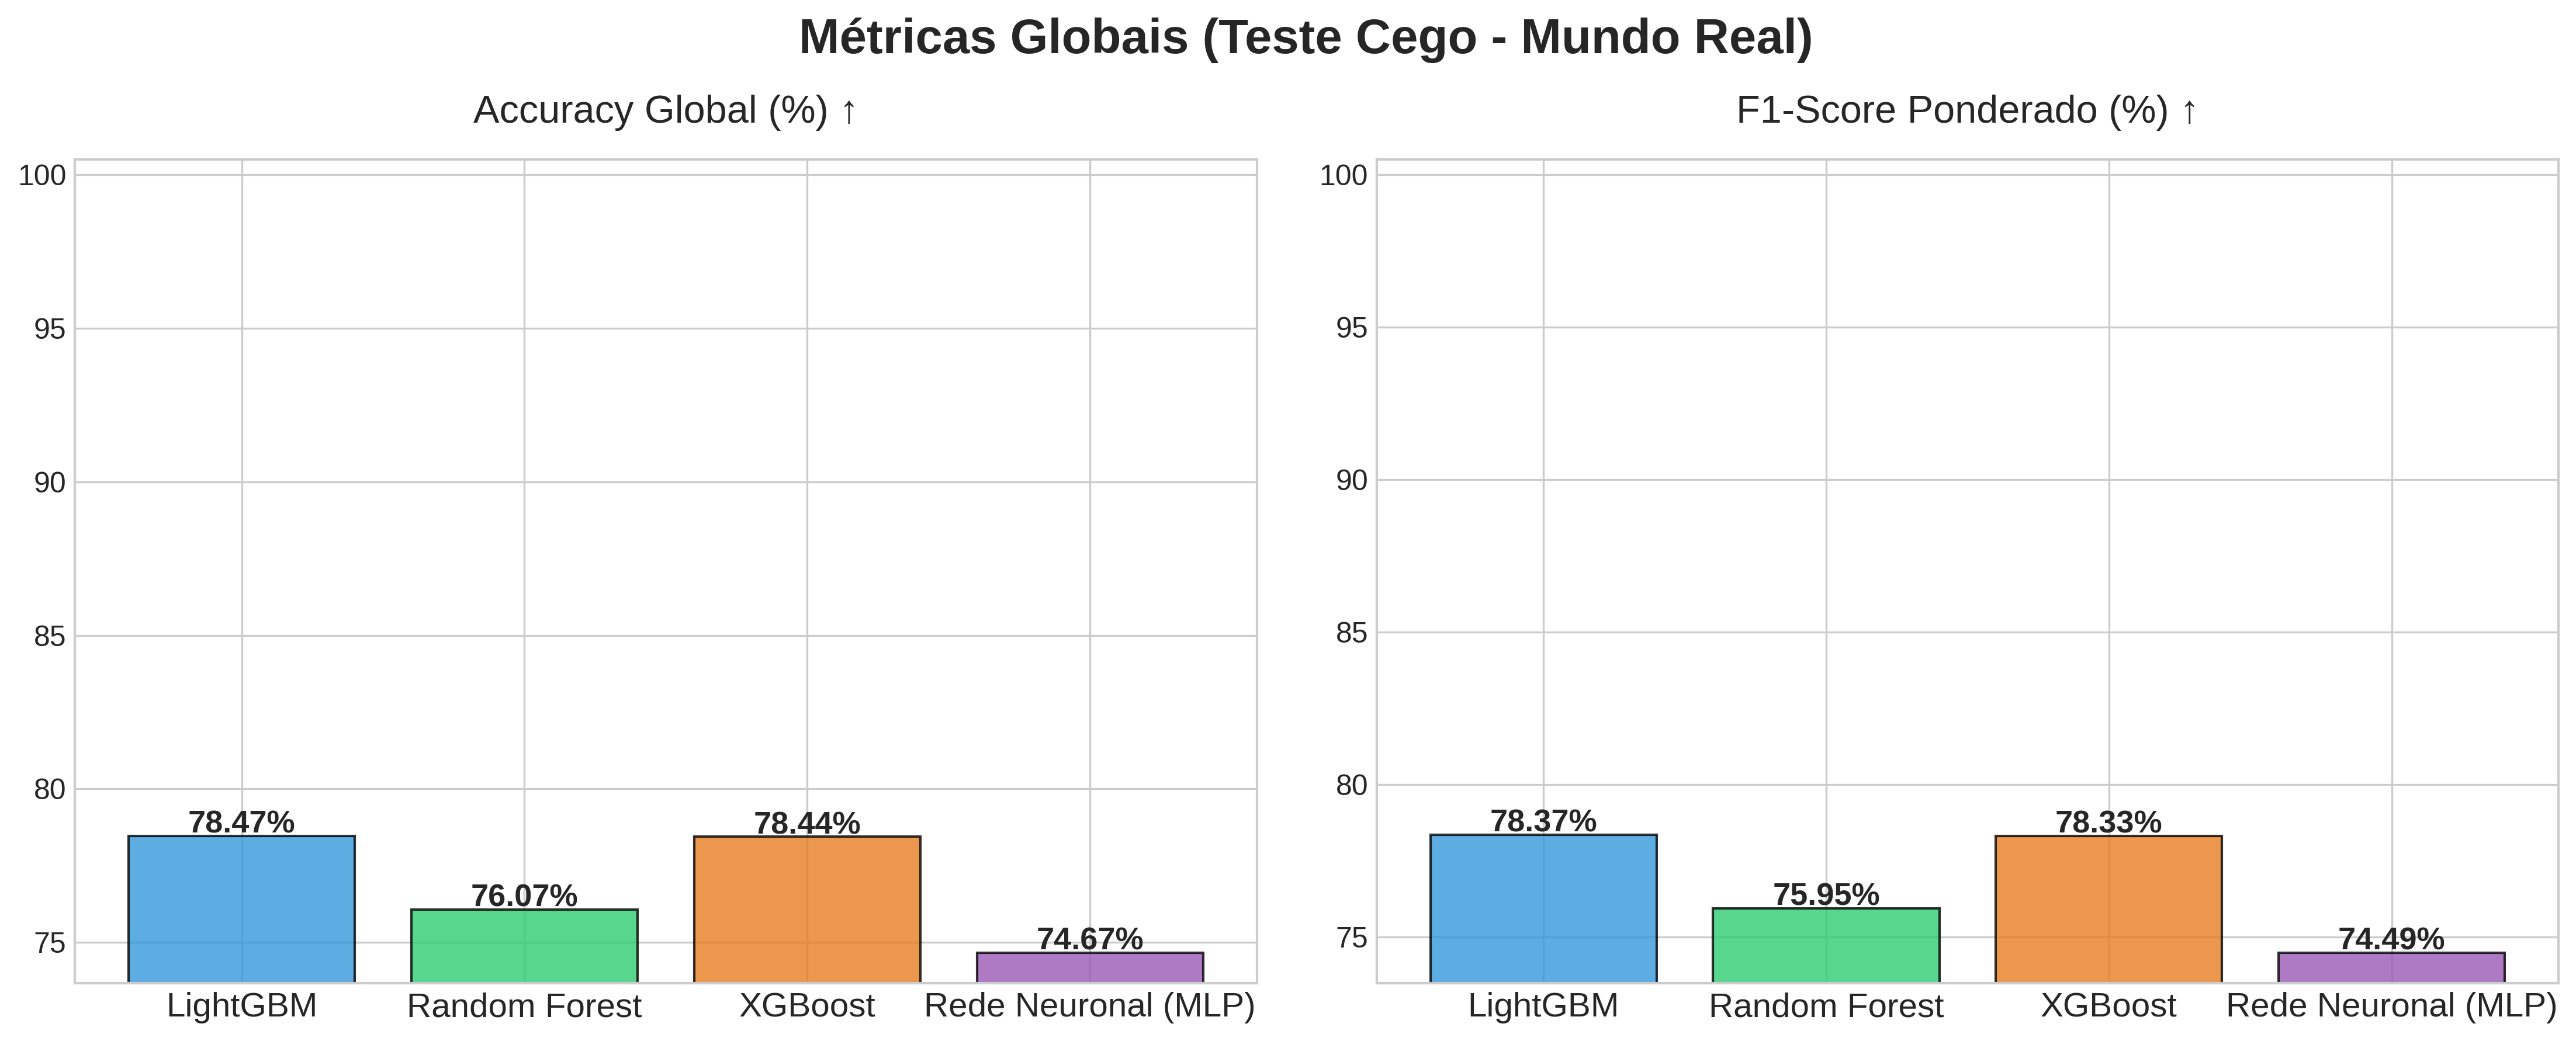
\includegraphics[width=0.9\textwidth]{imagens/grafico_teste_cego_global.png}
    \caption{Métricas Globais no Teste Cego - Mundo Real.}
    \label{fig:teste_cego_global}
\end{figure}

Observando os resultados, constata-se que o LightGBM e o XGBoost mantiveram-se como os modelos com melhor equilíbrio global em termos de precisão técnica, apresentando valores de F1-Score muito similares.

Contudo, para um cenário de \textit{Edge Computing}, a avaliação não se pode esgotar na precisão preditiva. A Figura \ref{fig:tempo_medio} ilustra o tempo médio que cada modelo requer para realizar a inferência de um único pacote.

\begin{figure}[H]
    \centering
    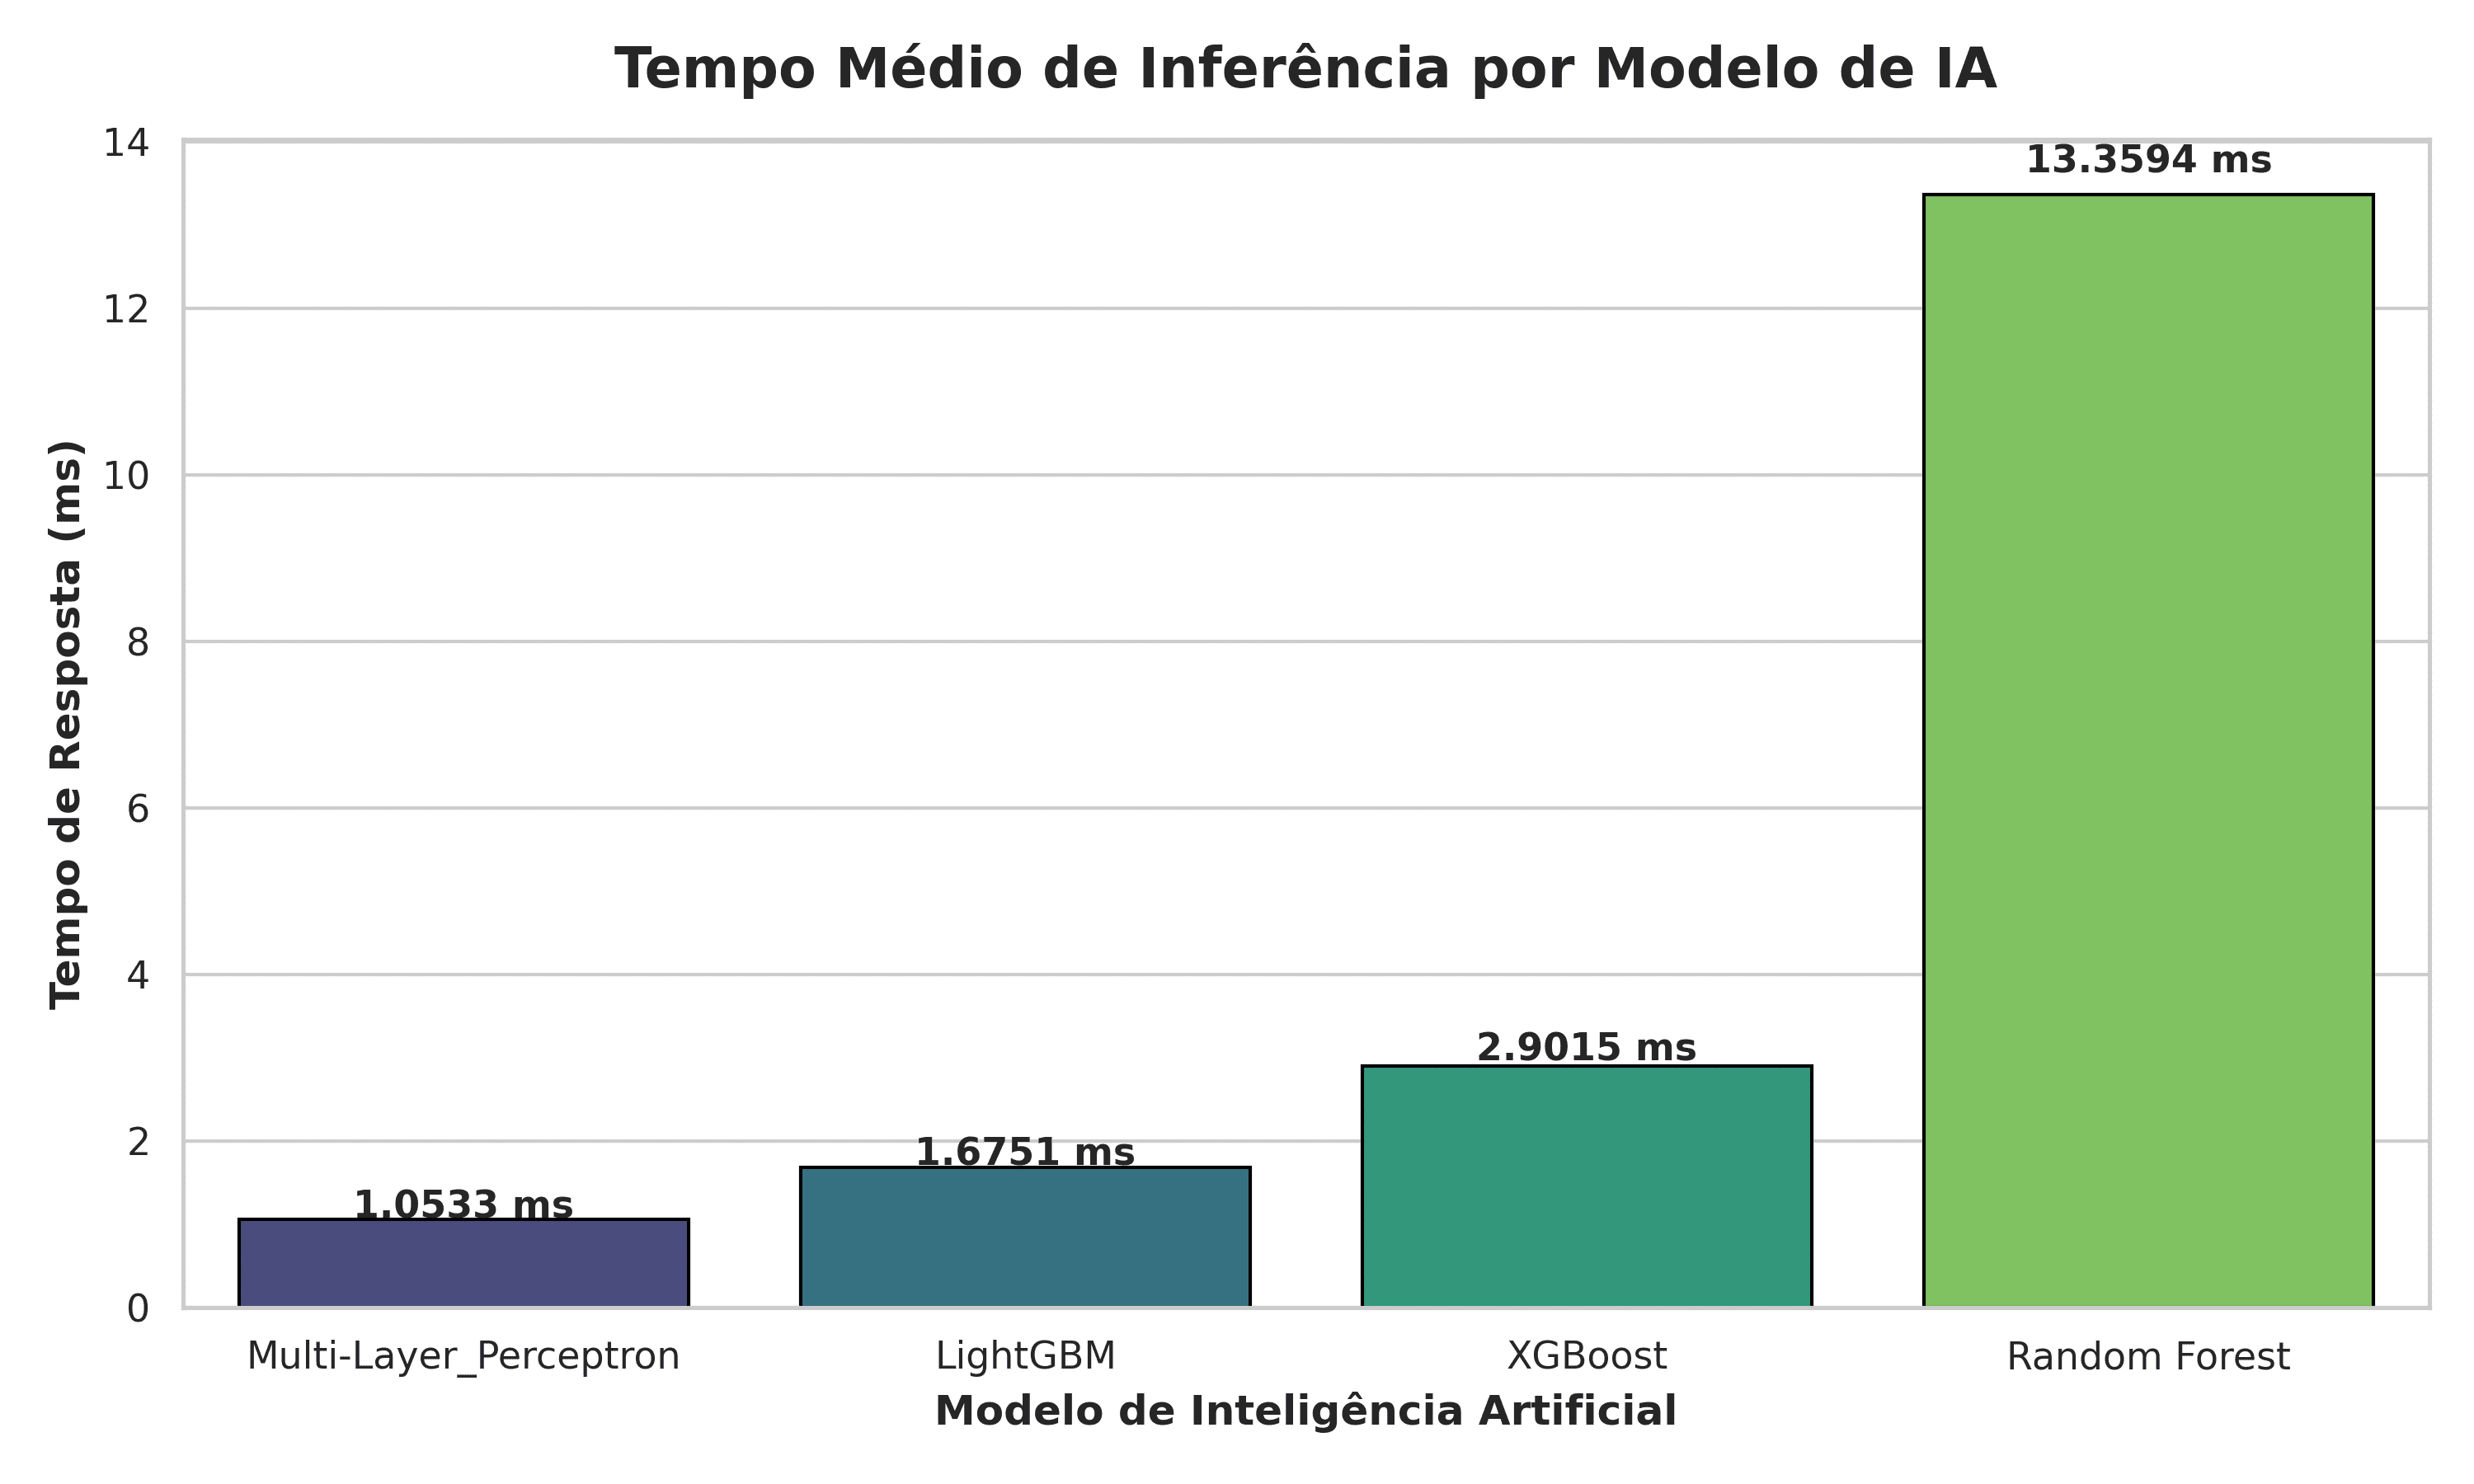
\includegraphics[width=0.85\textwidth]{imagens/grafico_tempo_medio_modelos.png}
    \caption{Tempo Médio de Inferência por Modelo de IA.}
    \label{fig:tempo_medio}
\end{figure}

Os dados da latência alteram drasticamente a perspetiva de viabilidade. Modelos profundos como o Random Forest apresentam latências inviáveis ($>13$ ms) para processamento em tempo real. Em contrapartida, a arquitetura matricial do Multi-Layer Perceptron (MLP) permitiu alcançar a maior velocidade operacional (pouco superior a 1 ms por pacote), revelando-se o algoritmo mais leve para atuar na periferia da rede. Esta estabilidade computacional do MLP, comparada aos restantes, é reforçada pela análise de variância da latência visível na Figura \ref{fig:boxplot_latencia}.

\begin{figure}[H]
    \centering
    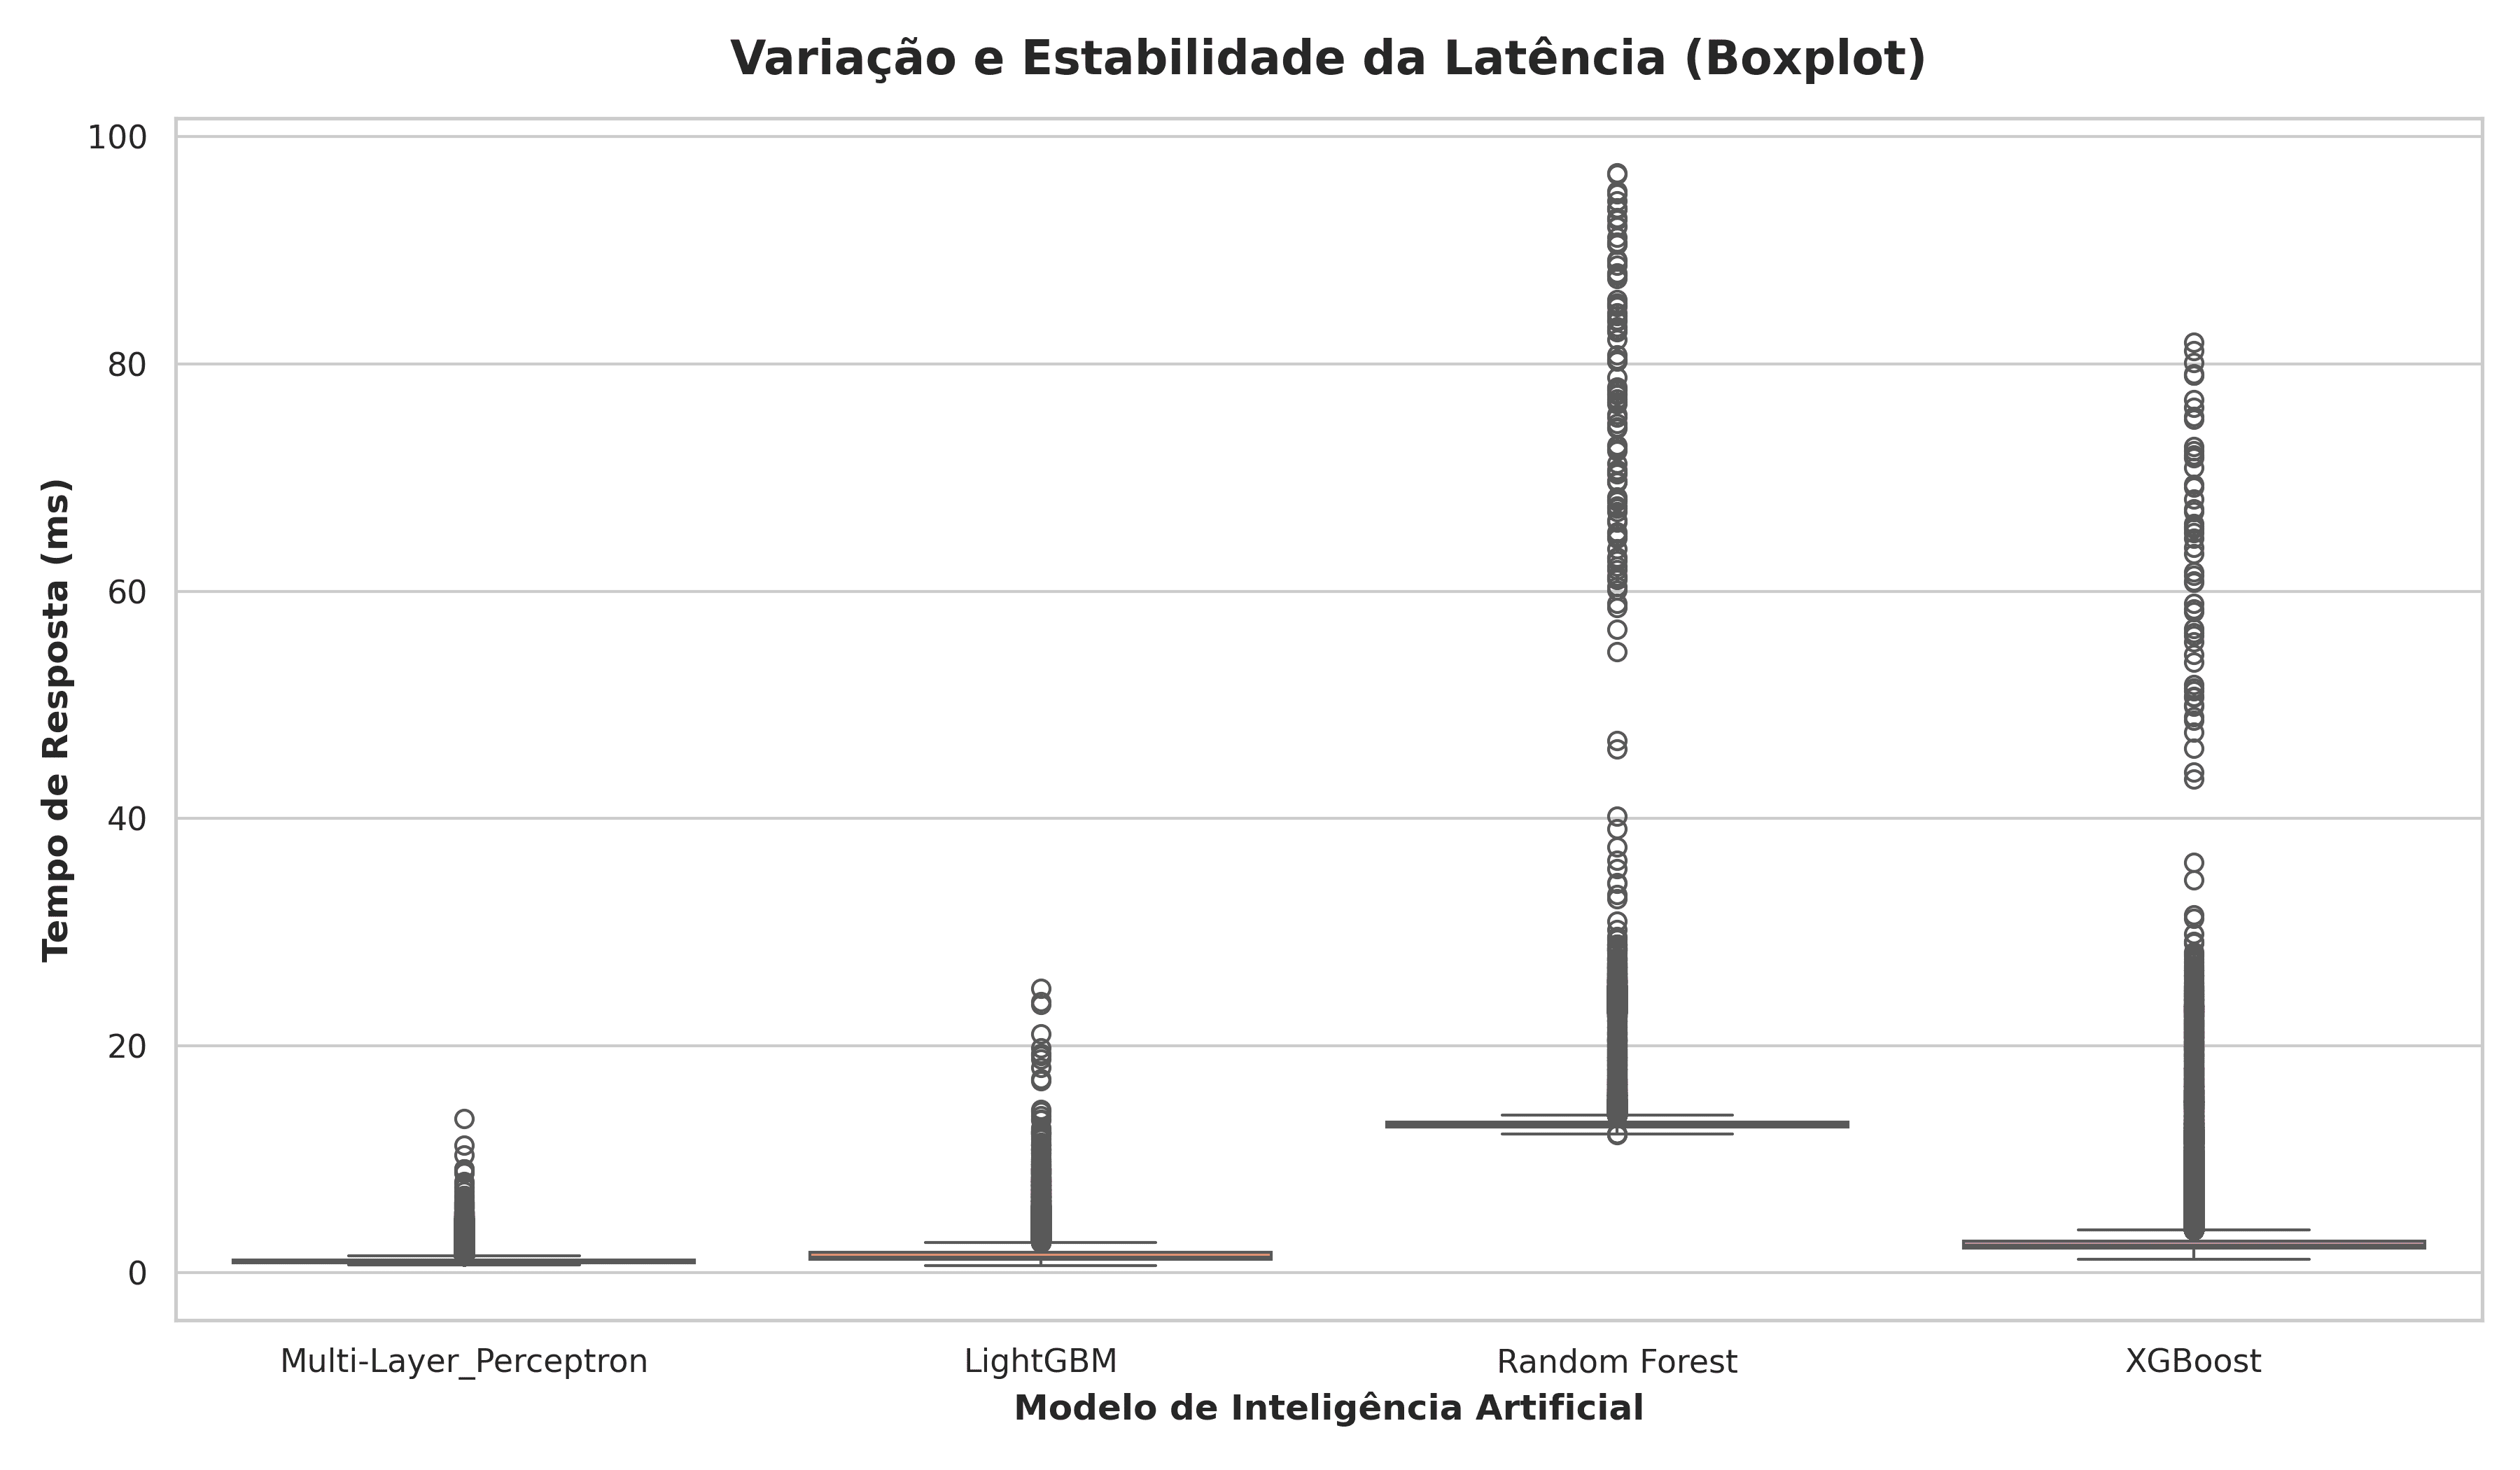
\includegraphics[width=0.9\textwidth]{imagens/grafico_boxplot_modelos.png}
    \caption{Variação e Estabilidade da Latência (Boxplot).}
    \label{fig:boxplot_latencia}
\end{figure}


\subsection{Recall por Anomalia}
\label{chap4:sec:recall_anomalia}

A análise da taxa de acertos por classe (Figura~\ref{fig:teste_cego_anomalias}) revela o
comportamento individual dos modelos perante cada tipo de ameaça e tráfego
legítimo, constituindo o indicador mais granular da robustez do sistema em
cenários reais.

\begin{figure}[H]
    \centering
    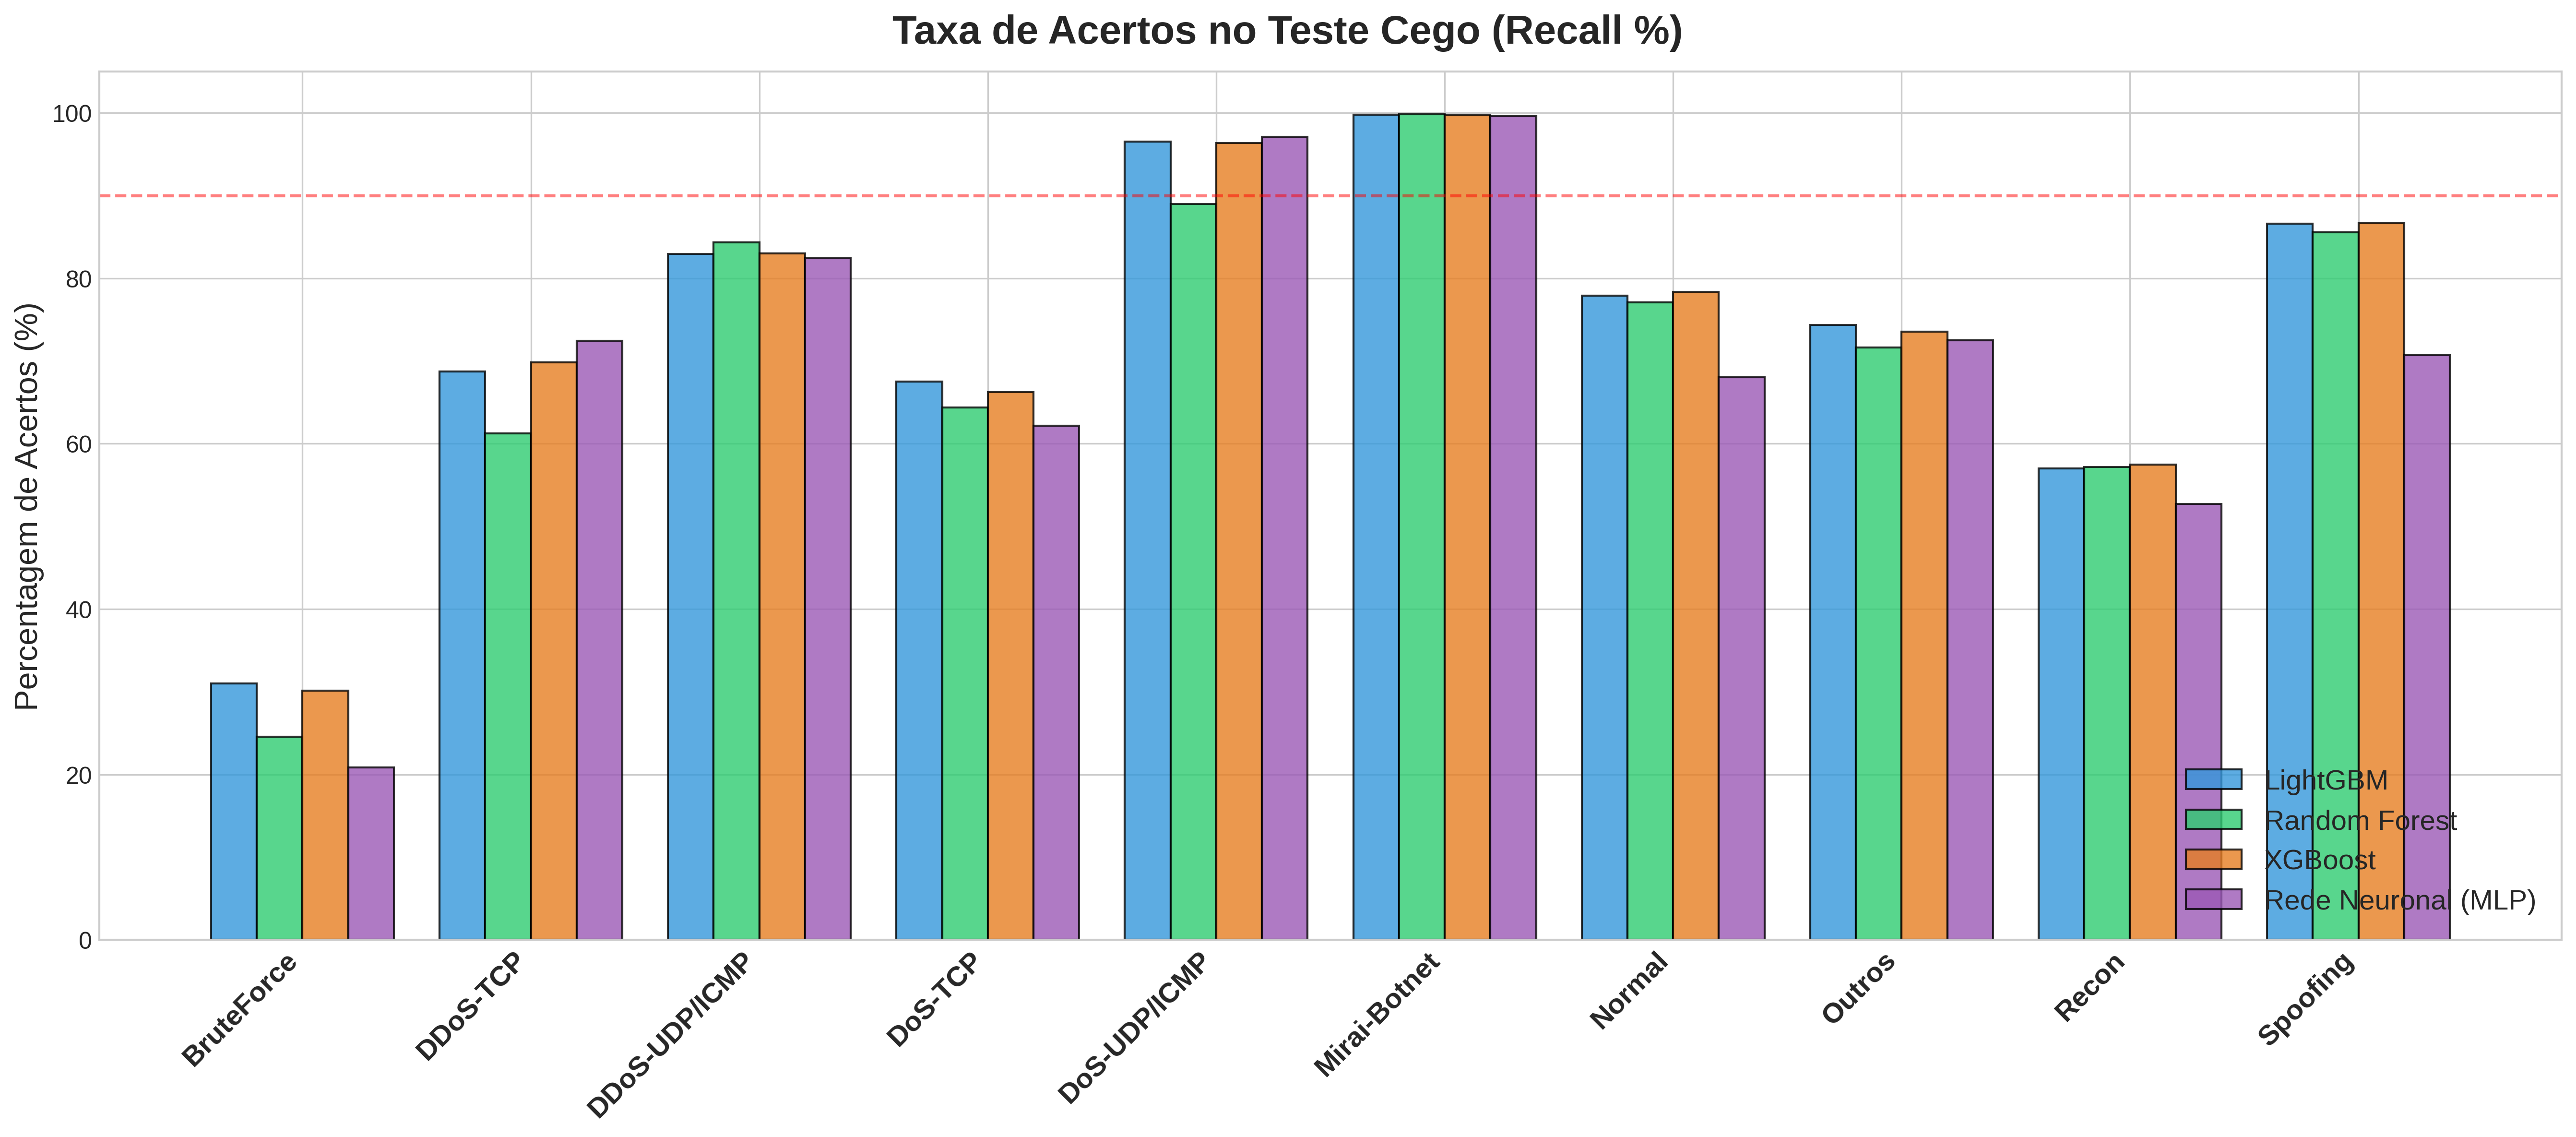
\includegraphics[width=0.95\textwidth]{imagens/grafico_teste_cego_anomalias.png}
    \caption{Taxa de Acertos (Recall \%) por Tipo de Anomalia.}
    \label{fig:teste_cego_anomalias}
\end{figure}


\textbf{Ataques Volumétricos (DDoS/DoS TCP e UDP/ICMP):} Todos os modelos
demonstraram um desempenho assinalável na deteção destas classes, com taxas
de \textit{Recall} próximas ou superiores a 80\%. A natureza volumétrica
e estatisticamente distinta destes ataques facilita a sua separação do
tráfego legítimo mesmo sem acesso ao \textit{payload}.

\textbf{Mirai Botnet e Spoofing:} Estas classes registaram igualmente
taxas de deteção elevadas, refletindo a agressividade dos padrões de
tráfego gerados por botnets, que produzem anomalias estatísticas facilmente
capturadas pela análise de fluxos.

\textbf{Tráfego Normal:} Todos os modelos garantiram uma taxa de permissão
de tráfego legítimo próxima dos 80\%, o que é crítico para evitar
interrupções de serviço causadas por falsos positivos numa infraestrutura
de \textit{Smart City}.

\textbf{BruteForce e Recon:} Estas duas classes apresentaram as taxas de
\textit{Recall} mais reduzidas entre todos os modelos avaliados. Esta
limitação é inerente à metodologia de extração de \textit{features}
baseada em fluxos estatísticos adotada: ataques furtivos como o
\textit{Recon} ou sessões de força bruta geram volumes de tráfego
reduzidos e padrões estatísticos subtis, que só seriam plenamente
distinguíveis através da Inspeção Profunda de Pacotes (DPI) ao nível
do \textit{payload}. Contudo, a adoção de DPI foi deliberadamente
excluída do âmbito deste projeto por incompatibilidade com os requisitos
de baixa latência e privacidade de dados impostos pelo paradigma de
\textit{Edge Computing}, conforme discutido na Secção~\ref{sec:ea_desafios_arquiteturais}.
Esta é uma limitação conhecida e aceite do sistema, cujo endereçamento
constitui uma das principais linhas de trabalho futuro propostas no
Capítulo~\ref{chap:conc-trab-futuro}.



\section{Decisão Final e Conclusões}
\label{chap4:sec:concs}

A seleção do algoritmo ideal para implementação num ambiente de \textit{Edge Computing} não se pode basear unicamente na maximização isolada da taxa de acertos. Exige, pelo contrário, uma avaliação rigorosa do compromisso (\textit{trade-off}) entre a eficácia preditiva e o custo computacional imposto ao \textit{hardware} da rede.

Conforme ilustrado na Figura \ref{fig:precisao_global}, os quatro modelos avaliados demonstraram níveis de exatidão global estatisticamente próximos, situados na faixa dos 74\% a 78\%.

\begin{figure}[H]
    \centering
    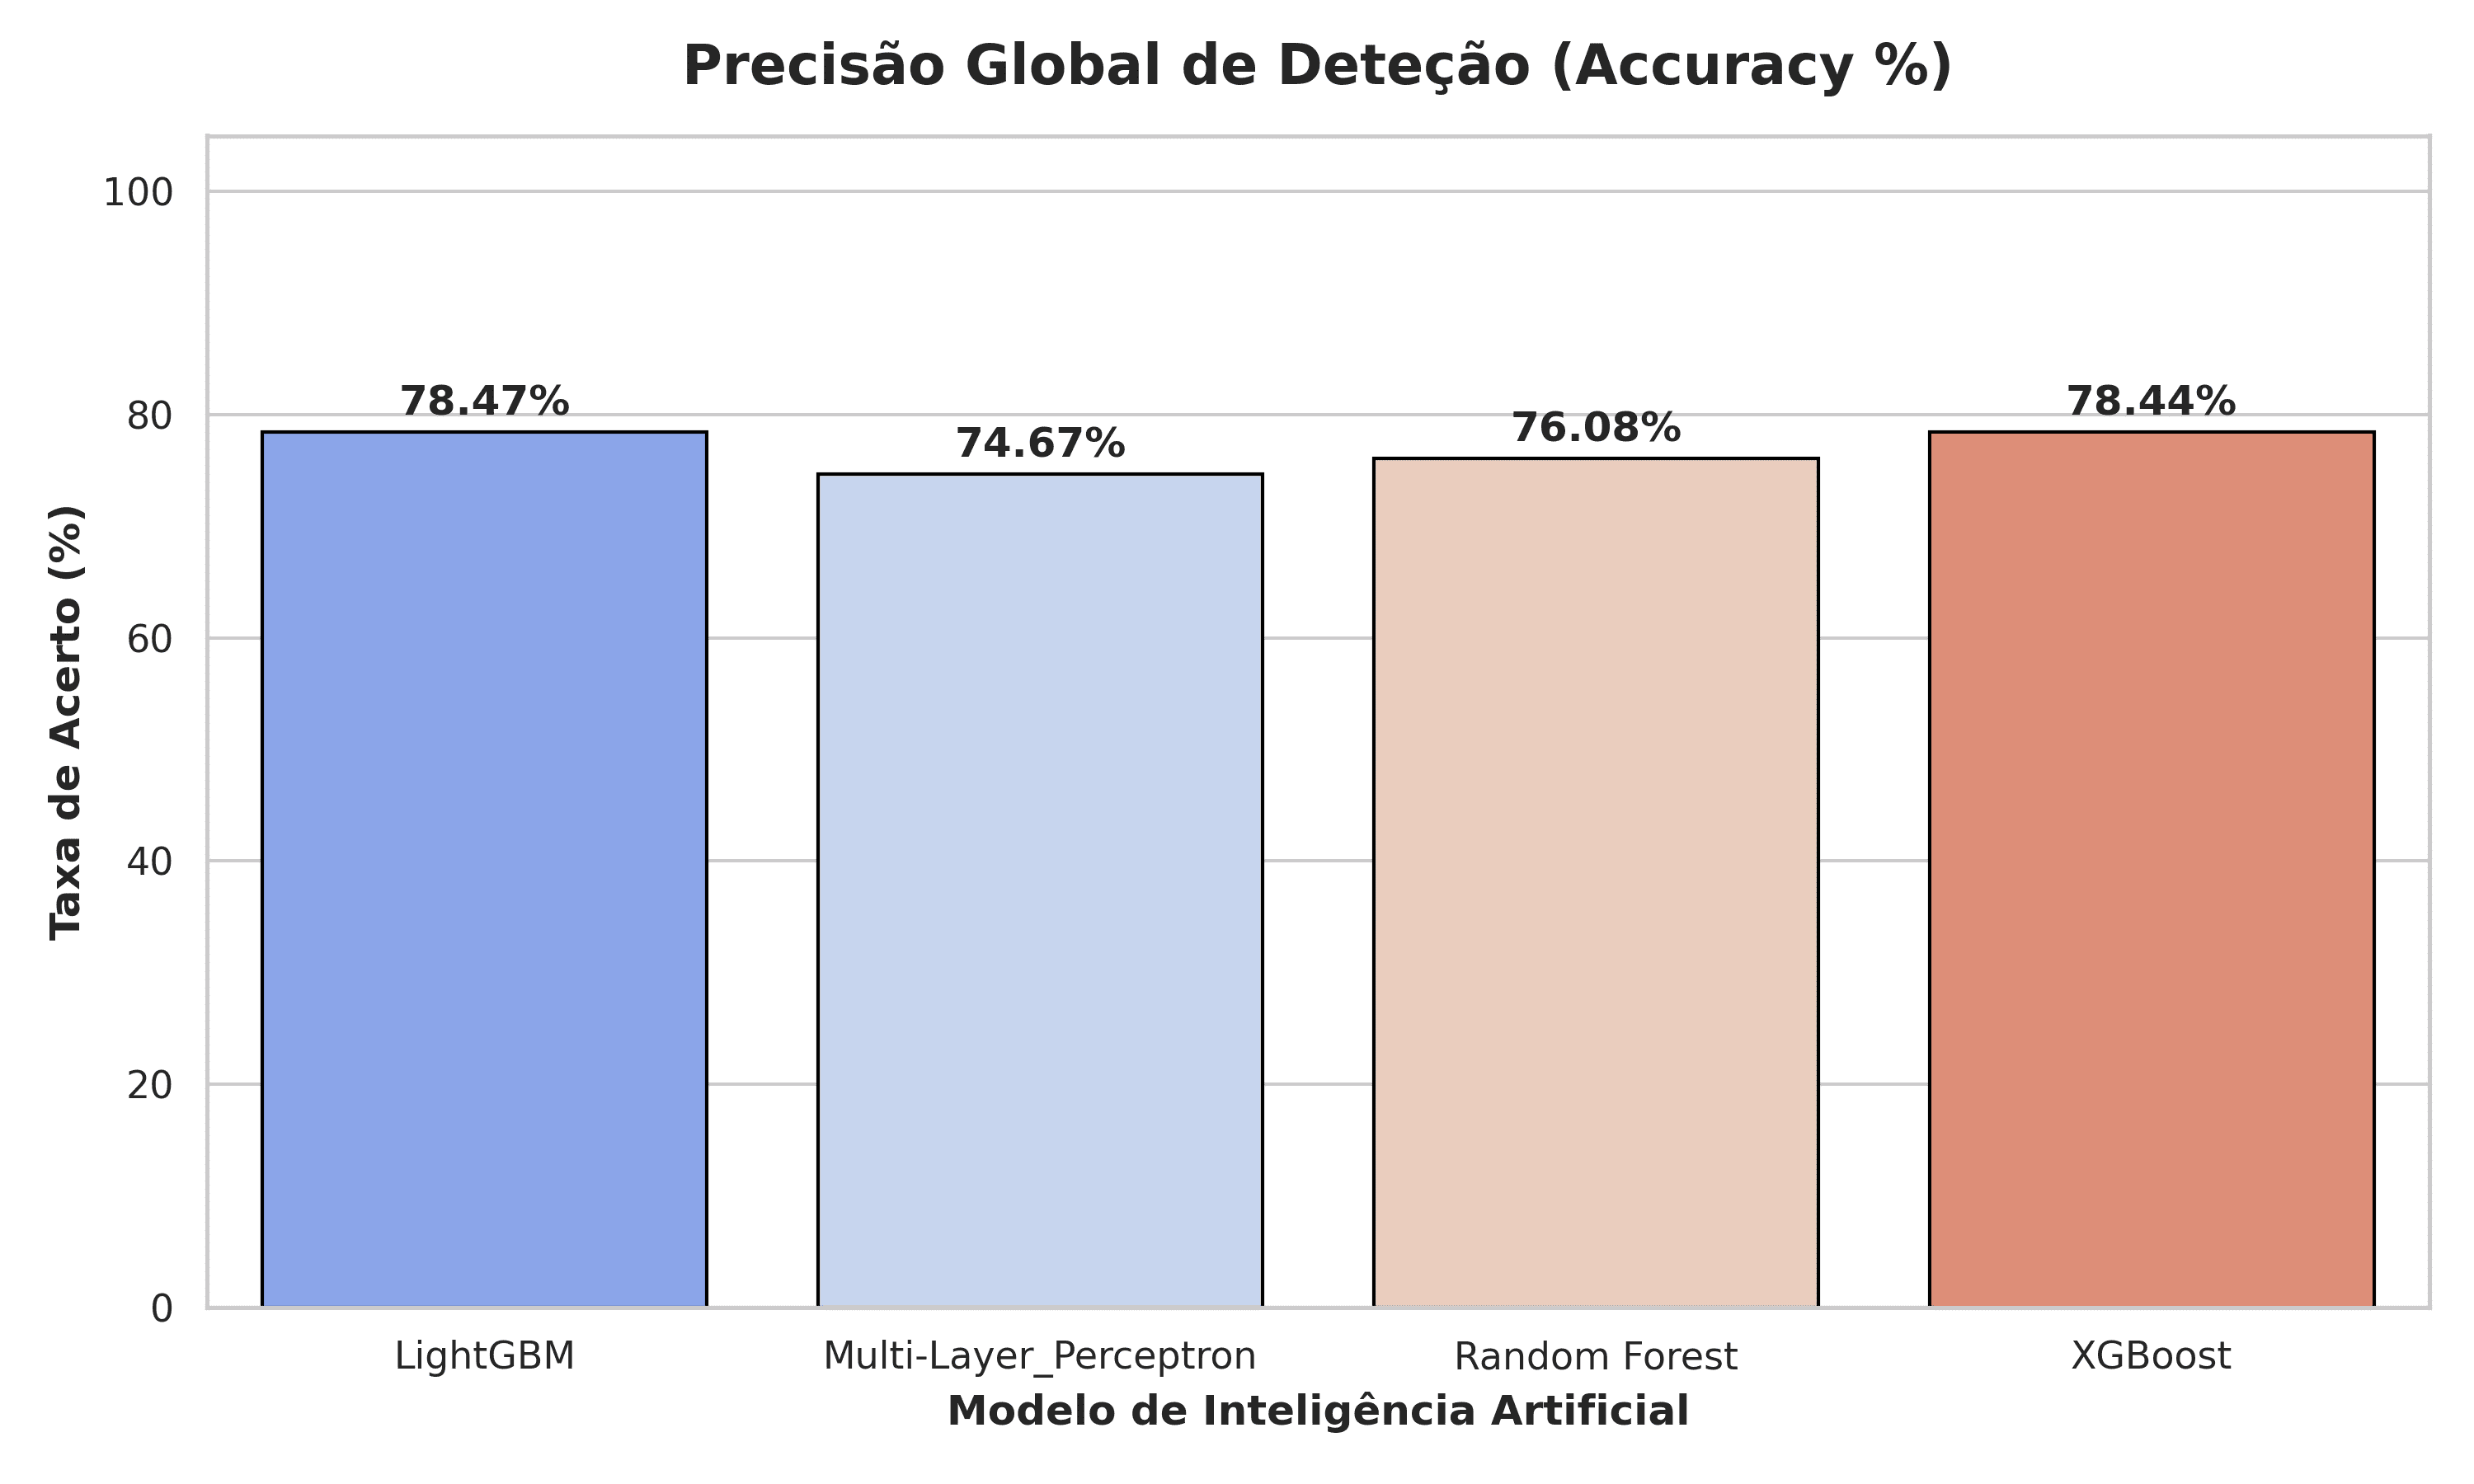
\includegraphics[width=0.85\textwidth]{imagens/grafico_precisao_modelos.png}
    \caption{Precisão Global de Deteção (Accuracy \%) por modelo.}
    \label{fig:precisao_global}
\end{figure}

No contexto das telecomunicações, mais crítico do que a latência média é a estabilidade desse tempo de resposta, vulgarmente conhecida por \textit{jitter}. A análise do \textit{Boxplot} na Figura \ref{fig:boxplot_latencia} revela que os modelos baseados em árvores (\textit{Random Forest} e \textit{XGBoost}) sofrem de uma elevada variância, apresentando picos anómalos de latência (\textit{outliers}) que chegam a atingir os 80 e 100 ms. Num \textit{Edge Router} sob o efeito de um ataque volumétrico massivo (DDoS), esta instabilidade provocaria o rápido esgotamento do \textit{buffer} de memória e o consequente bloqueio da rede (\textit{Denial of Service} autoinduzido). O MLP, por sua vez, destaca-se por uma variância praticamente nula, garantindo um comportamento predizível e determinístico sob stress de rede.

Adicionalmente, importa garantir que o tempo de processamento não sofre flutuações dependendo do ataque em curso. A Figura \ref{fig:tempo_por_classe} comprova que a latência do modelo MLP se mantém estritamente constante transversalmente a todas as anomalias. O esforço para aprovar um pacote legítimo (\textit{Normal}) é rigorosamente igual ao esforço para detetar um ataque furtivo (\textit{Recon}), prevenindo que atacantes explorem anomalias complexas para causar exaustão algorítmica no processador do \textit{router}.

\begin{figure}[H]
    \centering
    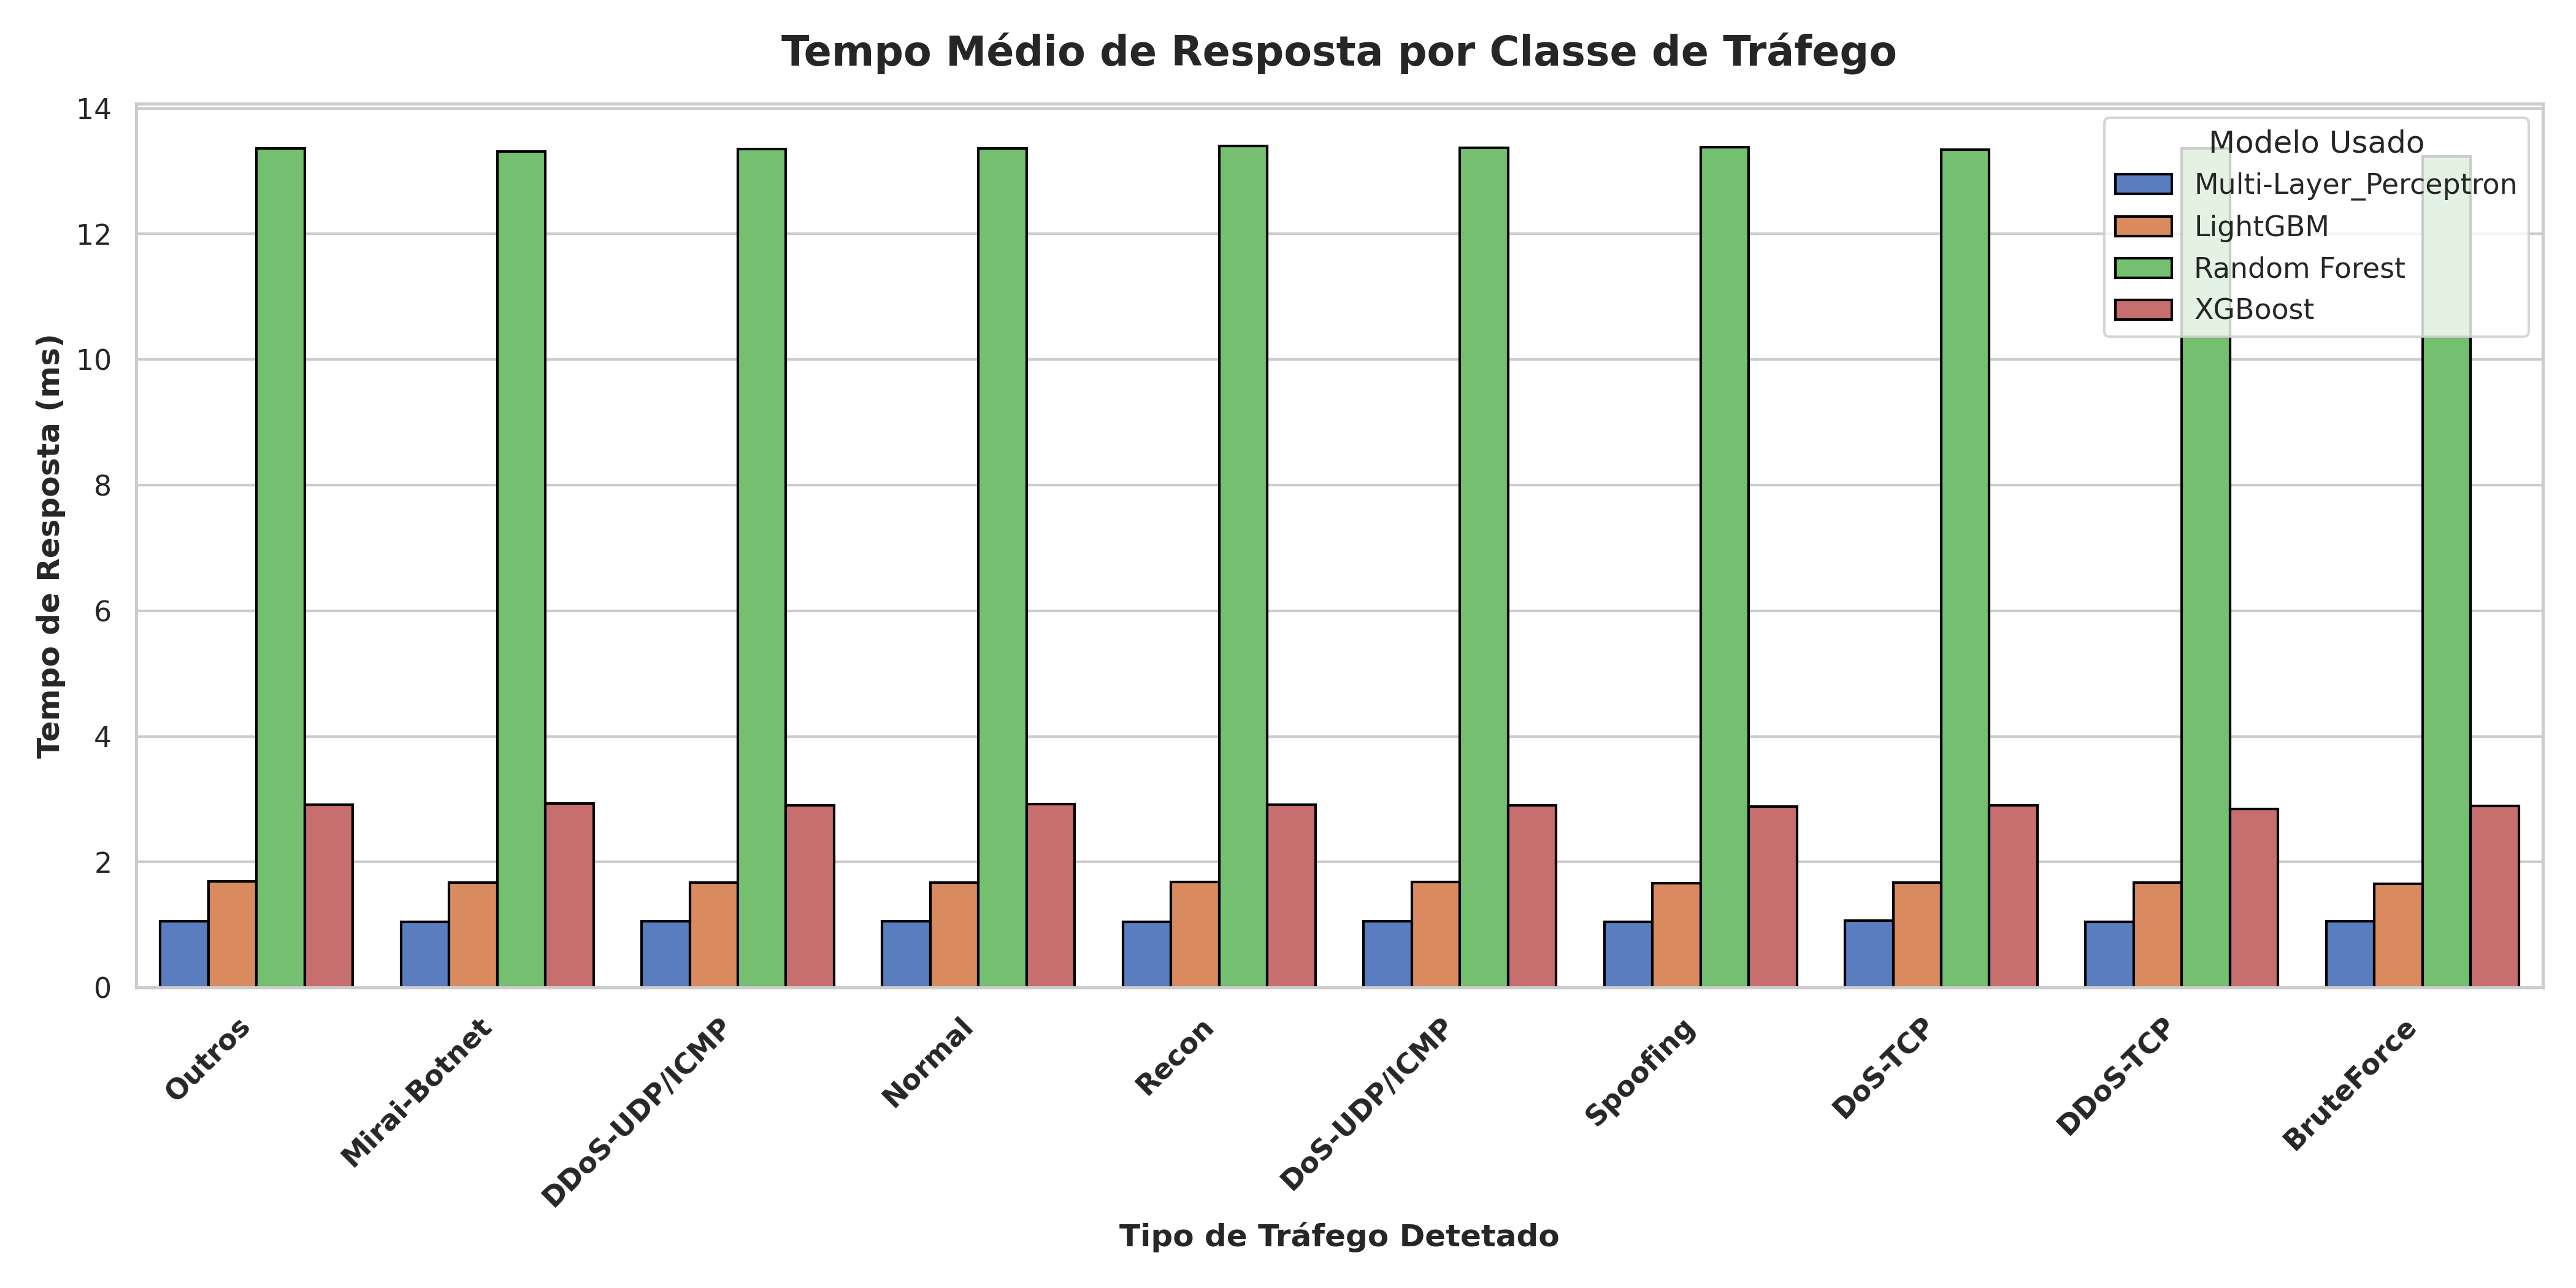
\includegraphics[width=0.9\textwidth]{imagens/grafico_tempo_por_classe.png}
    \caption{Tempo Médio de Resposta por Classe de Tráfego.}
    \label{fig:tempo_por_classe}
\end{figure}


\textbf{Conclusão:}
Perante a conjugação destas métricas físicas e lógicas, o \textbf{Multi-Layer Perceptron (MLP)} é declarado o algoritmo vencedor e o motor do sistema de segurança deste projeto. Embora ceda uma margem negligenciável na exatidão pura face ao \textit{LightGBM} (74,67\% vs 78,47\%), a sua velocidade operacional ultrarrápida ($\sim$1 ms) e estabilidade férrea garantem que o \textit{Edge Router} consegue mitigar pacotes em tempo real sem degradar a Qualidade de Serviço (QoS) da infraestrutura. Aliado ao mecanismo de \textit{Blacklist} Dinâmica, o modelo MLP confere ao sistema a escalabilidade perfeita para proteger ambientes de \textit{Smart Cities}.
